%% Manuscript for Computers & Geosciences (elsarticle class).
%% Every number is traceable through docs/traceability.md. Lines marked "AUTHOR CHECK" need
%% the authors' attention before submission.
\documentclass[preprint,12pt]{elsarticle}
\usepackage[T1]{fontenc}
\usepackage{lmodern}   % scalable (vector) fonts instead of bitmap EC fonts
\usepackage{amsmath}
\usepackage{graphicx}
\usepackage{booktabs}
\usepackage{lineno}
\usepackage[hidelinks]{hyperref}
\usepackage{xurl}      % lets long URLs break at any character
\emergencystretch=1.5em
\graphicspath{{../figures/}}
\journal{Computers \& Geosciences}

\begin{document}
\begin{frontmatter}

\title{Identifiability before interpretation: an inverse-crime test of physics-informed
petrophysical inversion across 625 wells of Mississippian chat}

\author[a]{Abrar Mahir\corref{cor1}}
\cortext[cor1]{Corresponding author. E-mail: [CORRESPONDING E-MAIL]}
\address[a]{[AFFILIATIONS]}

\begin{abstract}
Physics-informed neural networks are increasingly proposed for well-log interpretation without
core labels. We test how much such a label-free inversion can actually recover in a
low-resistivity chert reservoir, the Mississippian ``chat'' of Barber County, Kansas, using 625
wells of public Kansas Geological Survey logs. A coordinate-based neural field supplies spatially
varying rock-physics parameters (Archie exponents and a micro-porosity fraction), and
differentiable tool-response models reconstruct density, neutron, gamma-ray and resistivity logs
jointly. All decision rules were written down before the corresponding experiments. On synthetic
benchmarks the saturation exponent and the micro-porosity fraction were never recoverable. The
cementation exponent was recovered (correlation 0.87 to 0.93 with the truth) only when the
synthetic truth and the inversion shared one model family; when the truth came from a different
resistivity model the correlation fell to 0.15 to 0.60 and a null control with constant
cementation exponent returned a map with as much structure as a real one. The apparent success
was an inverse crime. In the pre-registered real-data test, production status of 378 producers
and 47 dry holes in spatially held-out blocks, the neural-field entries reached an area under the
curve of 0.643 and 0.573, significantly below a supervised baseline (0.780) and below the same
inversion applied well by well (0.726) and fixed-parameter Archie analysis (0.686). We conclude
that parameter maps from label-free physics-informed inversions should not be interpreted without
a model-mismatch test and null controls, and we release the complete pipeline, the decision log
and all results as an open benchmark.
\end{abstract}

\begin{keyword}
physics-informed neural networks \sep identifiability \sep inverse crime \sep well logs \sep
low-resistivity pay \sep negative results
\end{keyword}
\end{frontmatter}

\linenumbers

\section{Introduction}

Low-resistivity pay is a long-standing problem of log interpretation. In the Mississippian
``chat'' of south-central Kansas and northern Oklahoma, a porous weathered chert below the
basal Pennsylvanian unconformity, wells produce hydrocarbons from intervals whose deep
resistivity suggests water \citep{montgomery1998chat,watney2001chat,rogers2001chat}. Capillary
pressure data indicate abundant micro-porosity, which holds water that conducts current, and
the cementation exponent varies with facies \citep{watney2001chat,kgs2002chat}. Standard
\citet{archie1942} analysis with fixed parameters therefore mislabels pay as wet.
%% AUTHOR CHECK: the three AAPG papers and the KGS report were read as abstracts and web pages
%% only (see docs/literature_gap.md). Confirm these statements against the full texts.

Physics-informed learning \citep{raissi2019pinn} offers an attractive answer: put the
tool-response equations inside the network and learn from the logs themselves. Recent log
studies embed response equations in the architecture or the loss
\citep{pothana2025pinn,shao2024piml,tian2026satunn}, but they are trained with labels and
keep the rock-physics constants fixed. Label-free variants that reconstruct measurements
through a rock-physics decoder exist for seismic data \citep{vashisth2022rwpinn,li2024ppinn}.
Supervised models have been used to predict Archie exponents from logs and core
\citep{bagheri2026m,kumar2025n} and to flag low-resistivity pay \citep{gao2022lrlc}. Implicit
neural representations, or neural fields, are established for geological modelling and
geophysical inversion \citep{hillier2023geoinr,sun2023ifwi}. To our knowledge, no study has
represented the rock-physics \emph{parameters} themselves as a spatial neural field shared by
hundreds of wells and estimated them without core labels. That was the method we set out to
build.

This paper reports what happened when that method was tested rather than only demonstrated.
A label-free inversion has as many free quantities per depth sample as it has measurements, so
it can reproduce the logs almost perfectly whatever the parameters are. Whether the parameters
mean anything is a question of identifiability, and a synthetic test answers it only if the
synthetic data are not generated with the same model that is inverted, the ``inverse crime''
\citep{kaipio2007crimes}. Our contributions are:
\begin{enumerate}
\item an identifiability analysis of label-free physics-informed log inversion with decision
rules fixed in advance, including a demonstration that an apparently successful recovery of
the cementation exponent disappears under a change of model family;
\item a pre-registered test on real data, production status in spatially held-out blocks,
reported as a negative result;
\item an open, reproducible pipeline for 625 wells of public logs, with every decision,
result file and figure traceable.
\end{enumerate}

\section{Geological setting and data}

\subsection{Mississippian chat, Barber County}
The chat reservoirs of south-central Kansas lie beneath the Mississippian--Pennsylvanian
unconformity and combine high porosity with moderate permeability
\citep{montgomery1998chat,watney2001chat}. For the Glick field the Kansas Geological Survey
quotes cementation exponents averaging 2.36 and saturation exponents near 1.8
\citep{kgs2002chat}; we use the latter as the fixed saturation exponent.
%% AUTHOR CHECK: the Glick values are quoted from the KGS web report, which attributes them to
%% Duren (1967); the original was not seen and is not cited.

\subsection{Well logs}
All data are public records of the Kansas Geological Survey \citep{kgsdata}. A repackaged
copy on Kaggle (``Barber County Well Log Dataset (Kansas)'') was the starting point, but it
merges curves into one resistivity and drops matrix and caliper information, so we returned to
the original files. Of 1,054 Barber County LAS files in the survey index, 1,053 could be
downloaded and 1,050 parsed; they belong to 765 wells. Curve mnemonics were mapped to canonical
curves with a table built from the observed catalogue, units were harmonised, and files of the
same well were merged on a 0.5~ft grid.

The top of the Mississippian was taken from survey formation tops (615 wells) or, for 150 wells
without a pick, interpolated from the subsea tops of neighbouring wells by inverse-distance
weighting (leave-one-out mean absolute error 21~ft). A well is \emph{usable} if it has at least
20~ft of co-located gamma ray, bulk density, neutron porosity and deep resistivity inside the
Mississippian: 625 wells. Of these, 594 also have a shallow or medium resistivity, 259 a
photoelectric curve and 124 a sonic log; the latter two enter only as optional terms. Neutron
curves whose matrix is not stated were assumed to be in limestone units, because in 135 of the
136 wells that carry both a labelled and an unlabelled curve the two are identical. The analysis
window is the upper 100~ft of the Mississippian.

Descriptively, and only as motivation, wells recorded as Mississippian producers have a lower
median deep resistivity in the top 50~ft than dry holes (6.0 versus 9.8~ohm\,m; Mann--Whitney
$p = 2.6\times10^{-6}$).

\subsection{Labels and spatial blocks}
Labels were defined before any model was fitted: a \emph{producer} has an oil or gas status and
a Mississippian producing formation in the survey header (379 wells); a \emph{dry hole} has
status ``dry and abandoned'' (47 wells); the remaining 199 wells are unlabelled and are used
only by the label-free inversion. Because neighbouring wells are correlated, validation uses
spatially blocked cross-validation \citep{roberts2017cv}: 47 square blocks of 8~km were assigned
to five folds so that each fold holds 9 or 10 dry holes (Fig.~\ref{fig:map}). The split, the
well coordinates and the tops were frozen in a file before training.

\begin{figure}
\centering
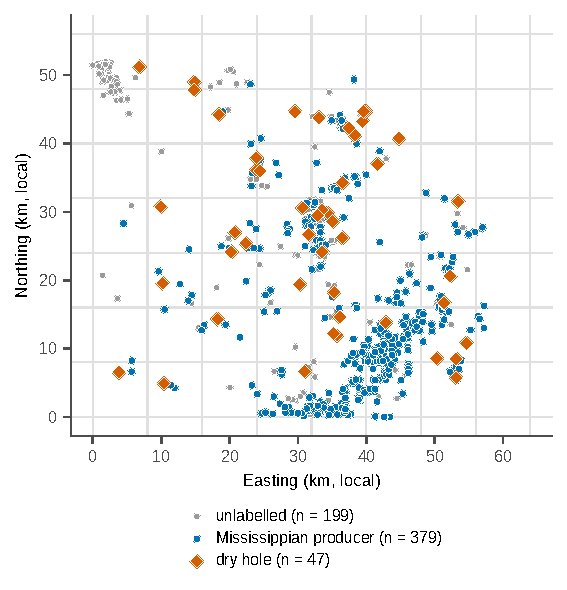
\includegraphics[width=0.6\textwidth]{fig1_wells_map.pdf}
\caption{The 625 study wells in local coordinates, with production labels and the 8~km blocks
used for spatially blocked cross-validation.}
\label{fig:map}
\end{figure}

\section{Method}

\subsection{Tool-response models}
Each sample is described by bulk-volume fractions that sum to one: total porosity $\phi$,
shale, and chert (quartz), calcite and dolomite. Bulk density and neutron porosity are linear
volumetric mixtures evaluated with the flushed-zone fluid; the photoelectric factor follows
from the volumetric cross-section; gamma ray is linear in shale volume with per-well
end-points; sonic slowness follows the time-average equation of \citet{wyllie1956} or a
velocity-average alternative. Deep resistivity $R_t$ reads the uninvaded zone and is modelled
either by \citet{archie1942},
\begin{equation}
R_t = \frac{a\,R_w}{\phi^{m} S_w^{n}},
\end{equation}
or by a parallel dual-porosity model in which a fraction $f$ of the porosity is micro-porous,
always water-filled, and conducts in parallel with macro-pores of water saturation $S_{w}$:
\begin{equation}
\frac{1}{R_t} = \frac{(f\phi)^{m}}{a R_w} + \frac{\left((1-f)\phi\right)^{m} S_w^{n}}{a R_w}
 + \frac{V_{sh}}{R_{sh}} .
\end{equation}
Shallow resistivity uses the same equations with mud-filtrate resistivity and a flushed
saturation $S_{xo}=S_w^{k}$ with a per-well exponent $k$. No environmental corrections are
applied; unknown corrections, calibration and the neutron matrix convention are represented by
per-well offsets with Gaussian priors. The relative pay indicator is the bulk volume of
hydrocarbon, $\phi\,(1-S_{w,\mathrm{total}})$, averaged over the window.

\subsection{Neural field and joint inversion}
A multilayer perceptron (four layers of 128 units) on Fourier features of the well coordinates
(six octaves) outputs the parameters $m$, $n$ and $f$ through bounded transforms, so that
parameters vary smoothly in space and are shared by all wells. The rock properties of every
sample are free variables. The loss is the masked Gaussian misfit of all available curves with
fixed noise scales, plus the priors on the per-well terms; noise scales are not learned, because
with free per-sample variables a learned variance collapses. Parameters are optimised with the
Adam algorithm and a cosine learning-rate schedule. Three variants differ only in how parameters
are tied: the spatial field, one free value per well (no sharing), and one global value. An
ensemble of ten random initialisations was run for every variant on real data.

For a held-out well the shared parts (field or global parameters, and one global $R_w$) are
frozen at their trained values and only per-sample and per-well terms are fitted. No production
label is used at any point by the inversion.

\subsection{Synthetic benchmarks}
Wells are scattered over an area of the size of the study area. Parameters are smooth random
fields, rock properties vary sample by sample with vertical correlation, and a hydrocarbon
column sits above a per-well contact. Three benchmarks were used.
\emph{v1} (60 wells) generates the logs with the same dual-porosity model that is inverted,
with noise, per-well offsets, the real curve coverage, an unknown flushing exponent and an
uncertain mud-filtrate resistivity.
\emph{v2} (200 wells) avoids the inverse crime: resistivity comes from a total-porosity model
of the \citet{waxman1968} type with an excess conductivity tied to micro-porosity, the neutron
response is non-linear, sonic uses a different transform, every curve carries per-well biases,
3\% of samples are washed out, and $R_w$ is unknown with a spatial trend.
\emph{v3} adds low-contrast dry wells: 10\% fully water-bearing and 15\% ``marginal'' wells with
residual hydrocarbon only.

\subsection{Decision rules fixed in advance}
All rules were committed to the public repository before the experiments they govern
(file \texttt{DECISIONS.md}, entries D20, D24a, D24b, D27, D28).
\begin{itemize}
\item \emph{Synthetic rule.} A parameter counts as recoverable if, in at least two of three
benchmark seeds, the correlation between recovered and true well values is at least 0.70 and
the root-mean-square error is at most half the true standard deviation (mean-centred in v2,
where only relative variation is claimed). A null control must also pass: when the true
parameter is constant, the recovered map must have a standard deviation below half that of a
real field.
\item \emph{Real-data rule.} The primary entry is the Archie neural field and the second entry
the dual-porosity neural field. The score is the area under the receiver operating
characteristic curve (AUC; \citealp{hanley1982auc}) for producers versus dry holes on wells of
held-out blocks, with stratified bootstrap intervals (2,000 resamples). Baselines are
fixed-parameter Archie and Simandoux-type analysis, the same inversion well by well and with
one global parameter, and two supervised classifiers (gradient boosting and a small
perceptron on per-well curve percentiles) trained on the labels of the training blocks. An
entry ``beats'' the best baseline only if the Bonferroni-corrected interval of the paired AUC
difference excludes zero. Otherwise the result is reported as negative.
\end{itemize}

\section{Results}

\subsection{Identifiability on synthetic data}
With truth and inversion in the same model family (v1), the cementation exponent passed the
rule narrowly (correlation 0.93, 0.87 and 0.92; error ratio 0.47, 0.57 and 0.41). The
saturation exponent and the micro-porosity fraction failed in every seed, and the null control
for $n$ failed: with constant true $n$ the recovered map had a standard deviation of 0.153
against a limit of 0.054 (Fig.~\ref{fig:ident}). Fixing $n$ changed nothing measurable, which
follows from the equations: $n$ only appears multiplied by $\log S_w$, and $S_w$ is itself free
at every sample.

Under the different-family truth (v2) the cementation exponent failed in all three seeds
(correlation 0.60, 0.15 and 0.50; centred error ratio 1.05, 1.48 and 1.30), and its null
control failed in all three (standard deviation 0.235, 0.166 and 0.245 against a limit of
0.106). A diagnostic run that kept every other difficulty of v2 but drew the truth from the
inverted model family recovered $m$ again (mean correlation 0.92). The model family alone
decides the outcome: the v1 success was an inverse crime. Two hundred wells instead of sixty
did not help, because the degeneracy is per sample. In v2 the total water saturation had a
root-mean-square error of about 0.2 and the estimated $R_w$ was biased low (0.024 against
0.042~ohm\,m), so absolute saturations and $R_w$ are not reported for real data.

\begin{figure}
\centering
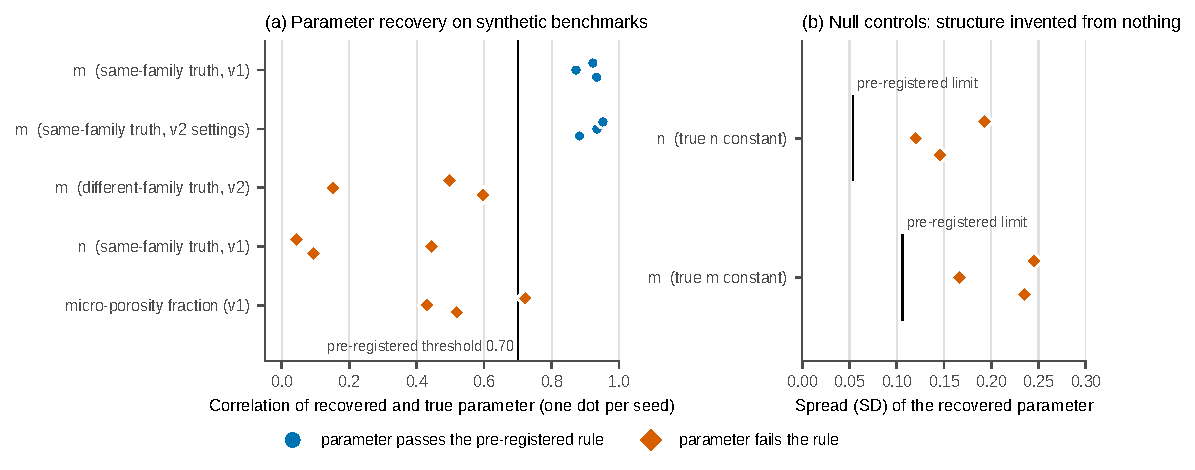
\includegraphics[width=\textwidth]{fig2_identifiability.pdf}
\caption{Identifiability on synthetic benchmarks. (a) Correlation between recovered and true
well-level parameters, one marker per benchmark seed; colour and shape give the verdict of the
pre-registered rule for the parameter, which also includes an error criterion (one
micro-porosity seed exceeds 0.70 but fails on error). (b) Null controls: spread of the recovered
parameter when the true parameter is constant, against the pre-registered limit.}
\label{fig:ident}
\end{figure}

\subsection{Pay indicator on synthetic data}
In v2 the bulk-volume hydrocarbon indicator correlated 0.87 to 0.93 with the truth at sample
level across model families, doubled noise and fixed $n$ between 1.6 and 2.2. Benchmark v3
showed that the well-level contrast in v2 had been easy: the AUC of the Archie field fell from
0.95 against fully wet wells to 0.86 against all dry wells including marginal ones
(Fig.~\ref{fig:synpay}). Field, well-by-well and global-parameter versions differed by 0.01 to
0.02, inside the seed-to-seed range, and fixed-parameter Archie analysis without any inversion
ranked wells slightly better (0.88). The dual-porosity inversion was no better than the Archie
inversion; its advantage in v1 was part of the same inverse crime.

\begin{figure}
\centering
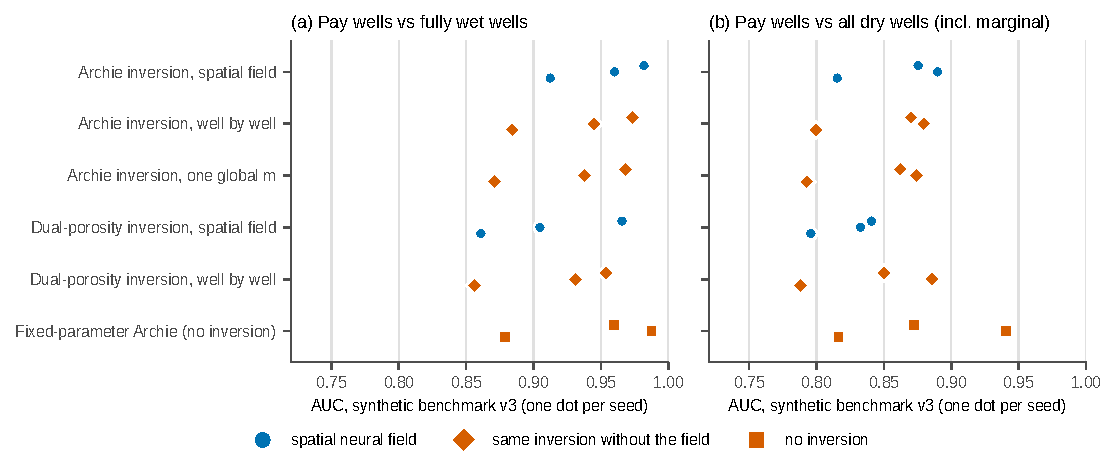
\includegraphics[width=\textwidth]{fig3_synthetic_pay_indicator.pdf}
\caption{Well-level AUC of the pay indicator on synthetic benchmark v3, one marker per seed:
(a) wells with a hydrocarbon column against fully water-bearing wells; (b) against all dry
wells, including marginal wells with residual hydrocarbon.}
\label{fig:synpay}
\end{figure}

\subsection{Pre-registered real-data test}
The test scored 378 producers and 47 dry holes (Table~\ref{tab:real}, Fig.~\ref{fig:real}). The
Archie neural field reached an AUC of 0.643 and the dual-porosity neural field 0.573. The best
baseline was supervised gradient boosting at 0.780. The paired differences were $-0.136$
(Bonferroni interval $-0.228$ to $-0.042$) and $-0.207$ ($-0.312$ to $-0.100$): both entries
are significantly worse than the best baseline, and the test is failed. The neural field was
also below the same Archie inversion applied well by well (0.726) and below fixed-parameter
Archie analysis (0.686).

The secondary test, predicting a hidden curve on held-out wells, failed as well. Relative to the
standard deviation of the hidden curve, the error was 0.81 to 1.10 for sonic, 1.33 to 1.45 for
the photoelectric factor and 1.9 to 3.6 for shallow resistivity, the latter with a bias of 0.5
to 1.1 decades. No variant predicted a hidden curve better than its mean.

\begin{table}
\centering
\caption{Pre-registered real-data test: AUC for producers versus dry holes on held-out spatial
blocks, with 95\% bootstrap intervals.}
\label{tab:real}
\begin{tabular}{lcc}
\toprule
Method & AUC & 95\% interval \\
\midrule
Supervised gradient boosting (best baseline) & 0.780 & 0.710--0.847 \\
Supervised perceptron & 0.764 & 0.688--0.838 \\
Archie inversion, well by well & 0.726 & 0.643--0.801 \\
Fixed-parameter Archie & 0.686 & 0.597--0.767 \\
Fixed-parameter Simandoux-type & 0.684 & 0.597--0.763 \\
Dual-porosity inversion, well by well & 0.660 & 0.572--0.745 \\
\textbf{Archie neural field (primary entry)} & \textbf{0.643} & 0.563--0.720 \\
Archie inversion, one global $m$ & 0.629 & 0.547--0.706 \\
\textbf{Dual-porosity neural field (second entry)} & \textbf{0.573} & 0.486--0.658 \\
\bottomrule
\end{tabular}
\end{table}

\begin{figure}
\centering
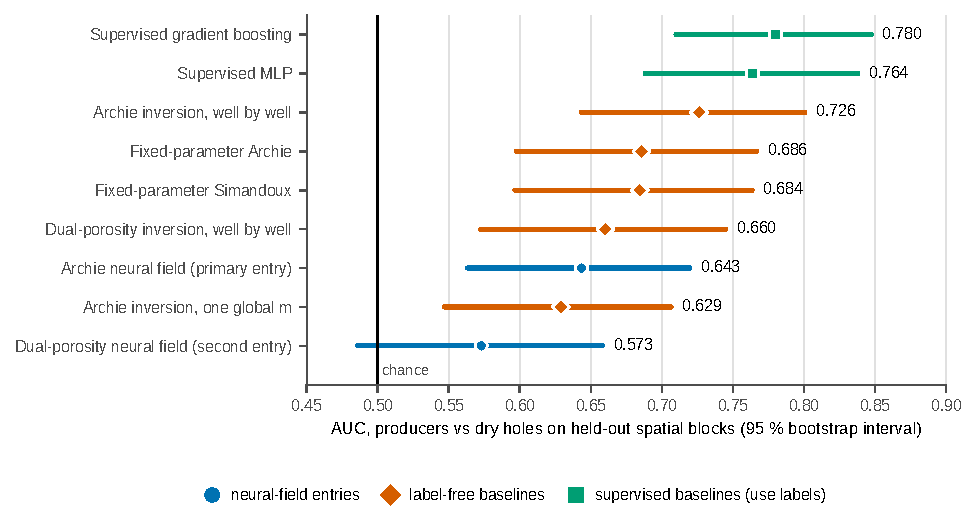
\includegraphics[width=0.85\textwidth]{fig4_real_data_auc.pdf}
\caption{Pre-registered real-data test (378 producers, 47 dry holes): AUC on held-out spatial
blocks with 95\% bootstrap intervals. The supervised baselines use production labels of the
training blocks; all other methods use no labels.}
\label{fig:real}
\end{figure}

\subsection{Exploratory observations (post hoc)}
The observations in this subsection were made after the test, from the saved outputs and
descriptive log statistics, without refitting anything. They are hypothesis-generating only.

\emph{Single raw statistics out-rank every inversion.} The mean density--neutron porosity of
the window alone gives an AUC of 0.755 and \emph{low} mean deep resistivity alone gives 0.745
(Fig.~\ref{fig:expl}b). Producers are the porous, low-resistivity wells. A saturation model
that reads low resistivity as water works against this signal, which may explain why adding
resistivity physics lowered the ranking below that of porosity alone.

\emph{Performance varies by area.} Across the five folds the AUC of the Archie field ranged
from 0.41 to 0.81 and that of fixed-parameter Archie from 0.47 to 0.93, whereas the supervised
model stayed between 0.63 and 0.80 (Fig.~\ref{fig:expl}a).

\emph{The ensemble has almost no spread.} The AUC of single ensemble members of the Archie
field lay between 0.642 and 0.645; different initialisations converge to the same solution.

\begin{figure}
\centering
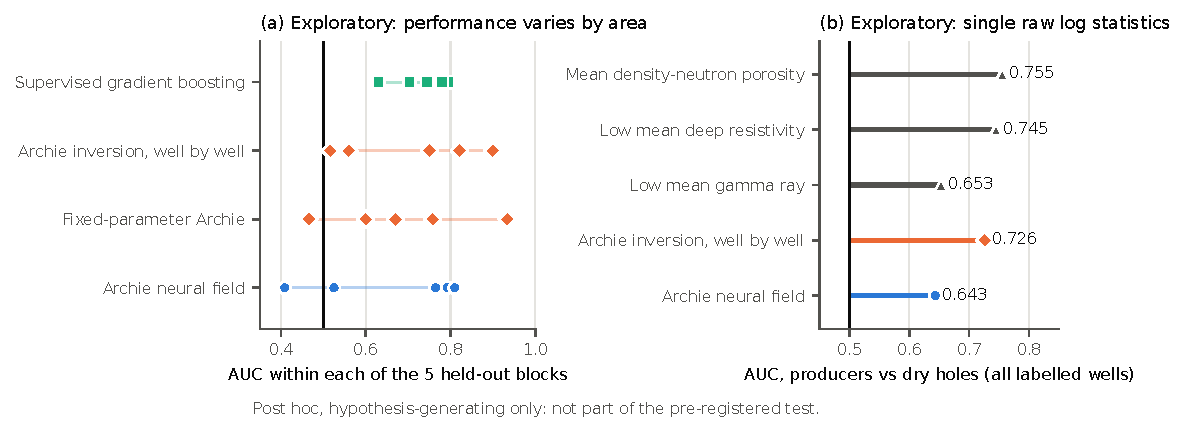
\includegraphics[width=\textwidth]{fig5_exploratory.pdf}
\caption{Exploratory, post hoc observations (not part of the pre-registered test). (a) AUC
within each of the five held-out folds. (b) AUC of single descriptive log statistics over all
labelled wells, compared with two inversions.}
\label{fig:expl}
\end{figure}

\section{Discussion}

\subsection{What the logs constrain}
The inversion fits the logs to within the assumed noise for any reasonable parameter values.
Goodness of fit is therefore no evidence for the parameters. In the same-family benchmark the
cementation exponent was constrained by the pair of deep and shallow resistivities, which share
$m$ but see different fluids; that constraint is real, but it is a property of the assumed
equations. Once the rock conducts differently from the model, the parameter absorbs the
mismatch and its map shows structure that is not in the rock. The null controls make this
visible and are cheap; we recommend them, together with a different-family truth, for any study
that interprets parameters estimated without labels.

\subsection{Why the neural field did not help}
Sharing parameters in space is only useful if the parameters are identifiable and vary smoothly.
The synthetic benchmark already showed no benefit of sharing; on real data sharing hurt. A
plausible reading, not tested here, is that parameters and the global $R_w$ learned on other
blocks transfer poorly to a held-out block, while the well-by-well inversion adapts to each
well. The supervised classifiers lead, but they answer a different question with production
labels; the informative comparison is among the label-free methods, where the neural field
is not the best either.

\subsection{Limitations}
\begin{itemize}
\item \emph{Identifiability.} $n$ and the micro-porosity fraction are not identifiable from
these logs; $m$ is model-dependent. No parameter map from this study should be interpreted.
\item \emph{Uncertainty.} The deep ensemble has almost no spread and is not a usable uncertainty
measure. The uncertainty that matters is between model families, which an ensemble of one
family does not capture.
\item \emph{Spatial heterogeneity.} Performance varies strongly by area (AUC 0.41 to 0.81
across folds for the primary entry), and with 47 dry holes the intervals are wide.
\item \emph{Labels.} Production status is a well-level label that also reflects completion
practice and economics, not only the rock; 378 of 379 producers were scored, because one has no
depth with density, neutron and deep resistivity together in the window.
\item \emph{No core comparison.} A comparison with the one public core analysis in the county
was not performed, because only well-level scores were saved from the registered run.
\item \emph{Tool physics.} The response models are simplified: linear neutron mixing, no
invasion or shoulder-bed modelling, textbook mineral end-points.
\item \emph{Environmental corrections and vintage.} Curves were used as delivered; corrections
applied by the contractors are unknown, mud-filtrate resistivities come from headers at surface
temperature, and the logs span several decades of tools (median spud year of the usable wells 2012). The neutron
matrix was assumed for 263 wells. Sensitivity to these factors was examined on synthetic data
only.
\item \emph{Absolute quantities.} Absolute water saturation and $R_w$ are not reported; the
benchmarks show they are biased.
\item \emph{Synthetic realism.} Even the different-family benchmark is far simpler than rock.
\item \emph{Literature.} The related work was assessed from abstracts and records; a full-text
survey may reveal closer precedents.
\item \emph{Pre-registration.} The rules were committed to a public version-controlled
repository with timestamps, not to an independent registry.
\end{itemize}

\section{Conclusions}
A label-free physics-informed inversion of well logs reproduced the logs and, on a benchmark
built with its own equations, appeared to recover a spatially varying cementation exponent.
Under a change of model family the recovery vanished and null controls showed invented
structure. On 625 real wells the neural-field pay indicator ranked producers and dry holes
worse than simpler label-free baselines and significantly worse than a supervised classifier.
For low-resistivity chert pay, the logs used here do not identify the Archie parameters
without independent calibration, and spatial sharing does not repair that. Different-family
benchmarks, null controls and decision rules fixed in advance should precede any geological
reading of parameters learned without labels.

\section*{Code availability}
Name of the code: \texttt{chert-pay-neural-field}. Contact: Abrar Mahir, [AFFILIATIONS], [CORRESPONDING E-MAIL].
Hardware: any CPU; the registered real-data run took about 12 hours on one consumer GPU.
Program language: Python 3.11 or later (PyTorch 2.15, NumPy, pandas, SciPy, scikit-learn,
lasio, Matplotlib). The source code, configuration files, decision log, result files and
figure scripts are available at
\url{https://github.com/abrarmahir31/chert-pay-neural-field} under the MIT licence
(documentation and figures: CC BY 4.0).
%% AUTHOR CHECK: add the tagged release and an archive DOI (for example Zenodo) at submission.

\section*{Data availability}
No raw data are redistributed. The well logs, headers, formation tops and core analyses are
public records of the Kansas Geological Survey; the repository contains a script that downloads
them from the survey servers and a data fingerprint that confirms an identical data set. The
source of this material is the Kansas Geological Survey website at
\url{http://www.kgs.ku.edu/}. All Rights Reserved.

\section*{Declaration of generative AI and AI-assisted technologies in the manuscript preparation process}
During the preparation of this work the authors used Claude (Anthropic), an AI system,
through the Claude Code agent, to write and run the analysis code, to search and verify the
literature, to draft the figures and to draft the text of this manuscript, under the authors'
direction and with decision points approved by the authors. The complete record of these
decisions is in the repository (\texttt{DECISIONS.md}). After using this tool, the authors
reviewed and edited the content as needed and take full responsibility for the content of the
published article.
%% AUTHOR CHECK: this is a DRAFT. Compare with the journal's current policy on generative AI,
%% which may restrict AI use beyond language editing; the extent of use here must be disclosed
%% accurately and the authors must have verified the code, results and text themselves.

\section*{CRediT authorship contribution statement}
Abrar Mahir: Conceptualization, Methodology, Investigation, Validation, Writing -- review \& editing, Supervision of the AI-assisted work. [AUTHOR CHECK: adjust the roles to what you actually did; see the AI declaration.]

\section*{Declaration of competing interest}
[To be completed by the authors.]

\section*{Acknowledgements}
We thank the Kansas Geological Survey for maintaining open access to well data.
[Funding statement to be completed by the authors.]

\bibliographystyle{elsarticle-harv}
\bibliography{references}

\end{document}
